\section{Benchmark Programs}
\label{sec:benchmark}
 
Besides the programs for transitive closure and vertex colouring, we select four more programs for benchmarking.


\subsection{Shortest distances}

\begin{tabular}{lp{10.5cm}}
\ul{Input:} & A graph $G$ with a unique grey node $s$. All edge labels are non-negative integers. \\
\ul{Output:} & The graph obtained from $G$ by marking grey each node reachable from $s$ and replacing its label $l$\/ with $l{:}d$, where $d$\/ is the shortest distance from $s$. (A distance is the sum of the edge labels of a directed path.)
\end{tabular}
  
\begin{figure}[htb]
\begin{center}
\input{Programs/distances.prog}
\end{center}
\caption{Program for shortest distances}\label{fig:shortest-distances}
\end{figure}

\ul{Notes}
\begin{enumerate}
\setlength{\itemsep}{-.5ex}
\item The result is unique up to isomorphism.
\item The input requirement can be relaxed by allowing negative edge labels but forbidding directed cycles with a negative distance.
\end{enumerate}


\subsection{Recognising acyclic graphs}
\label{sec:acyclic}

\begin{tabular}{lp{10.5cm}}
\ul{Input:} & Any graph $G$. \\
\ul{Output:} & Graph $G$ if it is acyclic, otherwise the program fails.
\end{tabular}
  
\begin{figure}[htb]
\begin{center}
\input{Programs/acyclic.prog}
\end{center}
\caption{Program for checking acyclicity}\label{fig:acyclicity}
\end{figure}

% \subsection{Rooted 2-colouring}
% 
% \begin{tabular}{lp{10.5cm}}
% \ul{Input:} & A connected graph $G$. \\
% \ul{Output:} & If $G$\/ is 2-colourable, then the output is obtained from $G$\% / by marking each node with either red or blue. The source and target of each % non-loop edge have different colours.\\
% & If $G$\/ is not 2-colourable, then the output is $G$.
% \end{tabular}
% 
% \vspace{10pt}
% \begin{tikzpicture} [scale=0.7,align=center,auto,inner sep=2mm,arrowin,arrowout,font=\ttfamily]
%init
\node at (0,0)[root,label=below:\scriptsize{1}]{x};
\node at (1.2,0){$\Rightarrow$};
\node at (1,0)[above=5mm] {init(x:list)};
\node at (2.4,0)[root,fill=red!75,label=below:\scriptsize{1}]{x};

%unroot
\begin{scope}[yshift=-3cm]
\node (l1) at (0,0)[root,label=below:\scriptsize{1}]{x};
\node at (1.2,0){$\Rightarrow$};
\node at (1.3,0)[above=5mm] {unroot(x:list)};
\node (r1) at (2.4,0)[inner sep = 2mm,circle,draw,label=below:\scriptsize{1}]{x};
\end{scope}


%make-red
\begin{scope}[xshift=5.5cm]
\node (l1) at (0,0)[root,fill=red!75,label=below:\scriptsize{1}]{x};
\node (l2) at (2.9,0)[inner sep = 2mm,circle,draw,label=below:\scriptsize{2}]{y}
   edge [-] node[above]{a} (l1);
\node at (4.1,0){$\Rightarrow$};
\node at (2.3,0)[above=5mm] {make-red(a,x,y:list)};
\node (r1) at (5.3,0)[circle,draw,fill=red!75,label=below:\scriptsize{1}]{x};
\node (r2) at (8.2,0)[root,fill=blue!60,label=below:\scriptsize{2}]{y}
  edge [-,dashed] node[above]{a} (r1);  
\end{scope}

%joined-reds
\begin{scope}[xshift=5.5cm,yshift=-3cm]
\node (l1) at (0,0)[root,fill=red!75,label=below:\scriptsize{1}]{x};
\node (l2) at (2.9,0)[circle,draw,fill=red!75,label=below:\scriptsize{2}]{y}
  edge [-] node[above]{a} (l1);
\node at (4.1,0){$\Rightarrow$};
\node at (2.6,0)[above=5mm] {joined-reds(a,x,y:list)};
\node (r1) at (5.3,0)[root,fill=red!75,label=below:\scriptsize{1}]{x};
\node (r2) at (8.2,0)[circle,draw,fill=red!75,label=below:\scriptsize{2}]{y}
  edge [-] node[above]{a} (r1);
\end{scope}

%back
\begin{scope}[xshift=2.75cm,yshift=-6cm]
\node (l1) at (0,0)[root,fill=red!75,label=below:\scriptsize{1}]{x};
\node (l2) at (2.9,0)[circle,draw,fill=blue!60,label=below:\scriptsize{2}]{y}
  edge [-,dashed] node[above]{a} (l1);  
\node at (4.1,0){$\Rightarrow$};
\node at (1.7,0)[above=5mm] {back(a,x,y:list)};
\node (r1) at (5.3,0)[circle,draw,fill=red!75,label=below:\scriptsize{1}]{x};
\node (r2) at (8.2,0)[root,fill=blue!60,label=below:\scriptsize{2}]{y}
  edge [-] node[above]{a} (r1);
\end{scope}

\end{tikzpicture}
 \\
% \vspace{10pt}
% 
% \ul{Notes}
% \begin{enumerate}
% \setlength{\itemsep}{-.5ex}
% \item The nodes in rule \ttt{unroot} are violet. They can match a node of any % colour. A violet right-hand node takes the colour of the match of the left-han% d node.
% \item The edges in the \ttt{mark}, \ttt{joined} and \ttt{back} rules are \emph% {bidirectional}. They match host graph edges in either direction.
% \end{enumerate}


\subsection{Generating Sierpinski triangles}

\begin{tabular}{lp{10.5cm}}
\ul{Input:} & A single node labelled with a non-negative integer $n$. \\
\ul{Output:} & The Sierpinski triangle of generation $n$.
\end{tabular}
  
\begin{figure}[p]
\begin{center}
\input{Programs/sierpinski.prog}
\end{center}
\caption{Program for generating Sierpinski triangles}\label{fig:Sierpinski-program}
 \begin{center}
  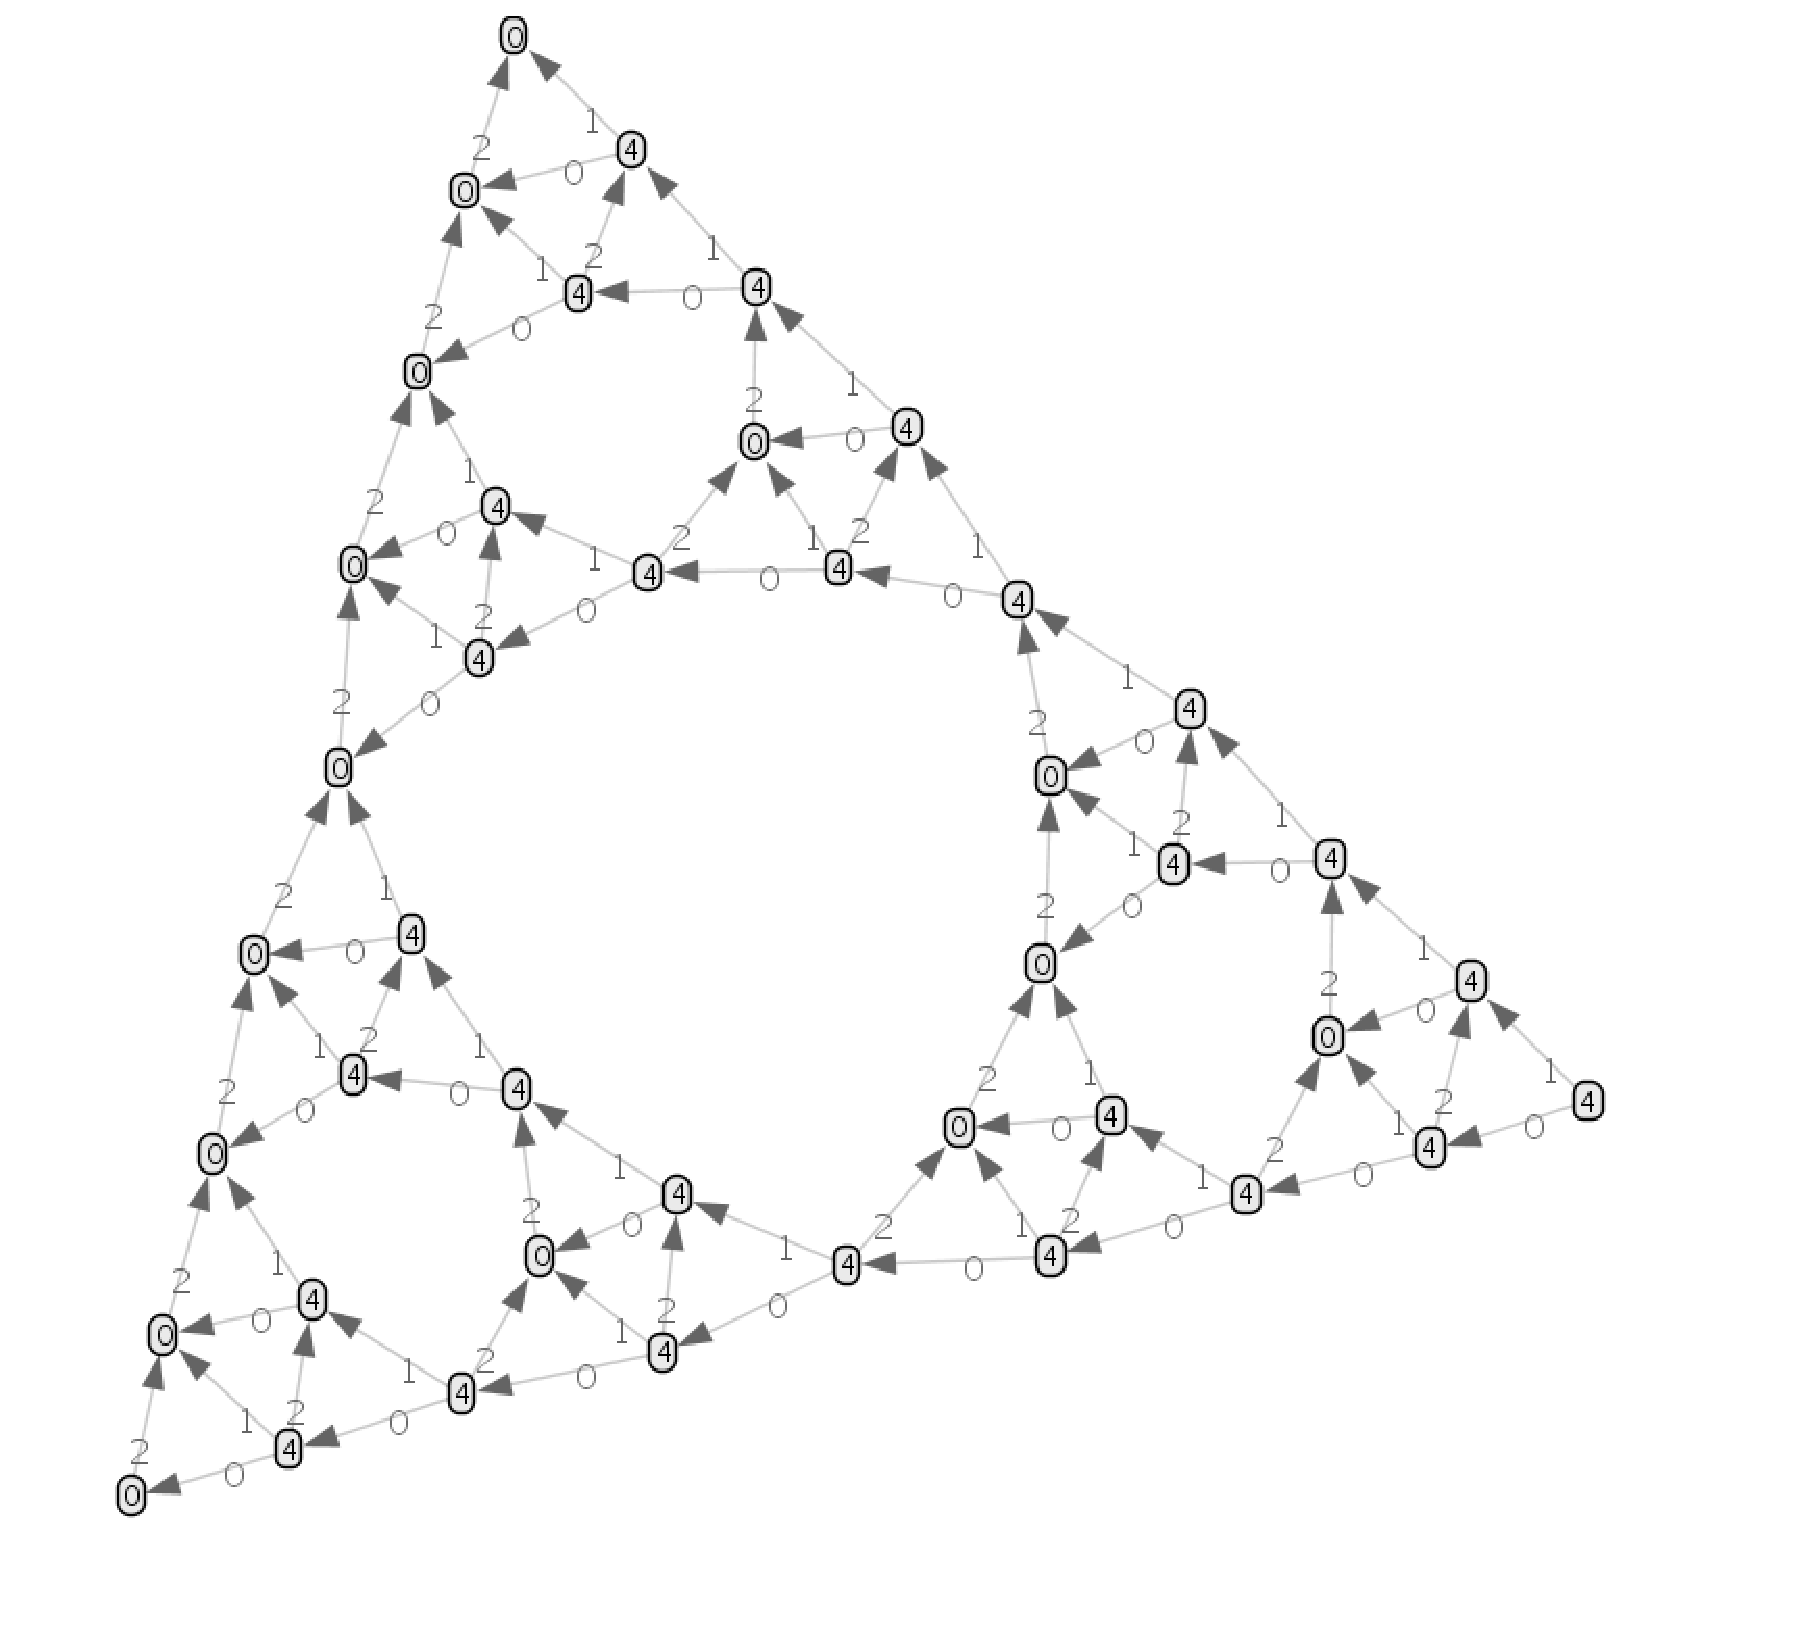
\includegraphics[scale=.35,angle=-15]{sierpinski-3.eps}
 \end{center}
\vspace*{-2.5cm}
\caption{Third generation Sierpinski triangle \label{fig:sierpinski}}
\end{figure}

\ul{Notes}
\begin{enumerate}
\setlength{\itemsep}{-.5ex}
\item The next page shows an example of a Sierpinski triangle.
\item The derivation length and the output size are exponential in $n$.
\end{enumerate}

Sierpinski triangles pose a hard challenge for graph transformation: generating the $n$-th triangle requires space and a number of rule applications exponential in $n$. This problem was part of the 2007 tool contest for graph transformation, where the goal was to generate triangles of generation numbers as high as possible and as fast as possible \cite{Taentzer_et_al08a}.
